%!TEX root =  ../main.tex

%https://numberwarrior.wordpress.com/2010/07/30/is-one-two-many-a-myth/
\begin{figure}
\begin{centering}
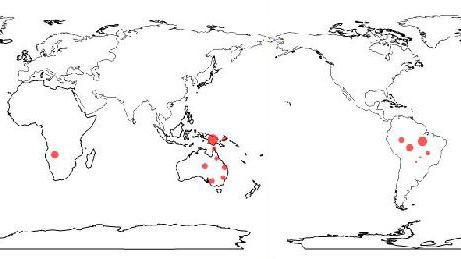
\includegraphics[scale=0.8]{twocounting1}
\caption[Languages with only two numbers]{The number of languages with only the numbers ``1'' and ``2'' (i.e., ``3'' == ``many'') is very few, but not zero.}
\end{centering}
\end{figure}

\subsection{Matching}

\objective{Understand and apply definitions of $\aleph_0$ and $\aleph_1$ to hypothetical problems involving infinity.}

\subsection{Countable Infinity}
There are the same number of: natural numbers, even numbers, odd numbers, integers and
rational numbers.  That may seem difficult to believe (surely there are half as many even numbers
as whole numbers!), but it is demonstrable.  We cannot count to infinity (by definition) so,
according to Georg Cantor, we must \emph{match} or pair element from one set to another.
If there exists a partner for every element of one set in another, with none left over, then
we can say the sets are the same size, even if they are infinite.

Now, consider the whole numbers, e.g. $0, 1, 2, 3, 4, \dots$.  While it would take an infinite 
amount of time to list them all (what Aristotle called a ``potential infinity'', meaning we can
conceive of how it potentially could be done), the whole numbers are conceivably countable,
so that infinity is called \textbf{countable infinity}.  Can we match the even up with them?
Yes!  Simply take each whole number, call it $n$, and map it onto $2n$, a unique even 
number.  This accounts for all of the whole numbers and all of the even numbers, so 
they are both countably infinite.  This infinity is called $\aleph_0$ (AL-eff NULL), because
it is the first infinity, and mathematicians start counting at zero.

It is each to see how the odds, the integers, and many other sets of numbers are also
of size $\aleph_0$, but things get trickier when we consider the rationals.  What does
your intuition tell you?  Cantor had to carefully construct a proof where he laid out 
all possible numerators in rows, and all possible denominators in columns.  By walking
diagonally through the list(s), he showed that it was possible to map the rationals
onto the wholes, and therefore they are the same size.

\begin{figure}[h]
\begin{centering}
\begin{tikzpicture}[myarrow/.style={red,->,shorten >=0.25cm, shorten <=.25cm}]
   \matrix (m) [draw,matrix of nodes,inner sep=.2cm,ampersand replacement=\&]
   {
    $\frac{1}{1}$ \& $\frac{1}{2}$ \& $\frac{1}{3}$ \& $\frac{1}{4}$ \& $\dots$\\
    $\frac{2}{1}$ \& $\frac{2}{2}$ \& $\frac{2}{3}$ \& $\frac{2}{4}$ \& $\dots$\\
    $\frac{3}{1}$ \& $\frac{3}{2}$ \& $\frac{3}{3}$ \& $\frac{3}{3}$ \& $\dots$\\
    $\frac{4}{1}$ \& $\frac{4}{2}$ \& $\frac{4}{3}$ \& $\frac{4}{4}$ \& $\dots$\\
    $\vdots$ \& $\vdots$ \& $\vdots$ \& $\vdots$ \& $\ddots$\\
   };
   \draw[myarrow] (m-1-1.center)--(m-2-1.center);
   \draw[myarrow] (m-2-1.center)--(m-1-2.center);
   \draw[myarrow] (m-1-2.center)--(m-1-3.center);
   \draw[myarrow] (m-1-3.center)--(m-2-2.center);
   \draw[myarrow] (m-2-2.center)--(m-3-1.center);
   \draw[myarrow] (m-3-1.center)--(m-4-1.center);
   \draw[myarrow] (m-4-1.center)--(m-3-2.center);
   \draw[myarrow] (m-3-2.center)--(m-2-3.center);
   \draw[myarrow] (m-2-3.center)--(m-1-4.center);
   \draw[myarrow] (m-1-4.center)--(m-2-4.center);
   \draw[myarrow,-,dotted] (m-2-4.center)--(m-3-3.center);
\end{tikzpicture}
\caption{Cantor's diagonal counting of the Rationals}
\end{centering}
\end{figure}

\subsection{Uncountable Infinity}
What about the irrational numbers?  Intuitively, you should see that there are more of
them, but intuition is not always trustworthy.  Every rational number is either a 
terminating or repeating decimal, but there can always be an infinity of irrationals
``in between'', with random digits.  Cantor employed another diagonal-type proof
in this case too, only now it will show a contradiction.

Suppose someone told you they had a list of all the irrational numbers, stored in 
some kind of crazy computer that could hold countably infinite number of numbers.
(A computer is convenient to bring into this story because computers store numbers
as 1's and 0's which makes this easier to demonstrate, but any list will do.)  Also
for simplicity's sake, let us just say we have listed all the irrationals from 0 to 1.
It is an infinite list of numbers, each with an infinite number of digits.


\begin{figure}
\begin{center}
  \begin{tabular}{ c | c c c c c c c c c  }
    \hline
    		& \textbf{0} & \textbf{1} & \textbf{2} & \textbf{3} & \textbf{4} & \textbf{5} & \textbf{6} & \textbf{7} & \textbf{8} \\ \hline 
    \textbf{0} & 0 & 1 & 0 & 1 & 0 & 0 & 0 & 1 & $\dots$ \\ 
    \textbf{1} & 1 & 1 & 1 & 0 & 1 & 0 & 1 & 1 & $\dots$ \\ 
    \textbf{2} & 1 & 0 & 0 & 1 & 1 & 1 & 1 & 0 & $\dots$ \\
    \textbf{3} & 0 & 1 & 1 & 0 & 0 & 1 & 0 & 0 & $\dots$ \\ 
    \textbf{4} & 1 & 0 & 1 & 0 & 0 & 1 & 0 & 1 & $\dots$ \\
    \textbf{5} & 0 & 1 & 1 & 1 & 0 & 0 & 0 & 0 & $\dots$ \\ 
    \textbf{6} & 1 & 1 & 0 & 0 & 0 & 1 & 1 & 0 & $\dots$ \\
    \textbf{7} & 0 & 1 & 0 & 1 & 0 & 0 & 0 & 1 & $\dots$ \\ 
    \textbf{8} & 0 & 0 & 1 & 0 & 0 & 0 & 0 & 0 & $\dots$ \\
    \textbf{9} & 1 & 1 & 0 & 1 & 0 & 1 & 0 & 1 & $\dots$ \\ 
    $\vdots$ & $\vdots$ & $\vdots$ & $\vdots$ & $\vdots$ & $\vdots$ & $\vdots$ & $\vdots$ & $\vdots$ & $\ddots$ \\
  \end{tabular}
\caption{A (supposed) list of all irrational binary numbers.}
\end{center}
\end{figure}

Now suppose I am a rather incorrigible bloke, and I come along an make a
number not on the list.  To do that, let us consider the main diagonal of the
list, i.e. coordinates (0,0, (1,1), (2,2), (3,3), etc.  Because this list in in binary 
(1's and 0's), it is very easy to make that place on my \emph{new} number
the opposite of whatever was on the list.  My new number is infinitely long, and
differs from every number on the original list in at least one decimal place, by
definition.  You might even add my number to the list, but I can do the same
process again and create a new number not on \emph{that} list.  I have
proven that the list of irrationals --- even just between 0 and 1 --- is \emph{not}
listable, and \textbf{uncountable infinity}.

The Reals, the Irrrationals, and other sets have a size we must notate as
$\aleph_1$ (AL-eff sub WUHN).




